\chapter{Theory}
\label{theory}

\minitoc

In this chapter theory and literature relevant to the study is presented. It starts of with an introduction of both traditional and agile software development methodologies, with the main focus on Scrum. Afterwards a shift towards coordination is taken. Some well-known literature is looked at, for example Malone and Crowston's coordination theory. Further, to put the study into context, a definition of large-scale is given. To end the chapter a look at different aspects of effectiveness in team coordination is introduced.

\newpage

\section{Software Development Methodologies}

The term software development methodologies has been around for quite some time now. These methodologies are frameworks for accomplishing a well-structured development process. In this section a brief introduction to the most prominent methodologies will be carried out. It will start with a quick look at the traditional software development, before ending with a presentation of the new and agile way of thinking. In the last section (on agile software development) the main focus will be on Scrum as this is the methodology found in most of the literature gathered from the literature review.

\subsection{Traditional Software Development}

Traditional software development methodologies have a distinct pattern. This pattern is sometimes called software development life cycle (SDLC) methodologies which is often found in system engineering. These ``life cycles'' are in contrast to the ``iteration''-approach found in agile methodologies, such as Scrum. The most well-known of these traditional software development methodologies is Waterfall discussed further below.

\subsubsection{Waterfall}

The Waterfall methodology is one of the classic development models. It was first described in a paper by W. W. Royce in 1970 \cite{waterfall}.  The model was not yet named in this paper, which it received later mostly due to its iconic structure (as shown in figure \ref{waterfall}).

In the aforementioned paper, it is suggested that all software development models tend to go through two distinct phases: Analysis and Coding. The author argues that it is not possible to write a software project without having a somewhat deep understanding of the underlying problems that it needs to solve. Therefore an analysis phase will always be required in advance of writing the program itself. However, he also mentions that such a simple model is only suitable for programs that are completed in a matter of days. Larger software projects require an extended number of steps.

For larger projects, the following steps are suggested:
\begin{enumerate}
	\item \textbf{System and Software Requirements:} The customer is involved with the specification of the scope and requirements of the system. The resulting documentation serves as a foundation to the next stages of development.
	\item \textbf{Analysis and Program Design:} The requirements produced in the previous stage are used to create a system plan and various design documents.
	\item \textbf{Coding and Testing:} The actual implementation of the project. This also involves continuously testing on various levels (for example unit and integration).
	\item \textbf{Operation and Maintenance:} Once the project has been completed, it has to be maintained during its usage. In addition to improving the program in various ways, this may also involve the inclusion of extra features if the customer so desires. These features can in themselves use the Waterfall model.
\end{enumerate}

\begin{figure}
\centering
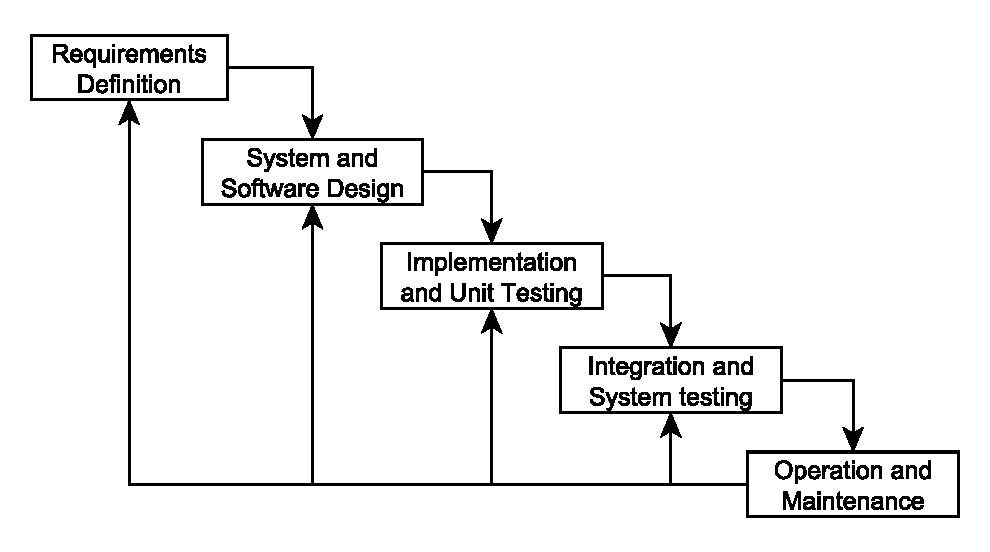
\includegraphics[width=150mm]{images/chapters/development_models/waterfall.pdf}
\caption{The Waterfall model.}
\label{waterfall}
\end{figure}

The model initially suggested by W. W. Royce discusses a linear model in which each of the aforementioned stages are used as distinct steps in the development process. Each stage is required to be completed before the next is started. This may be a sound premise in theory, but as suggested in the paper it is likely to fail in practice. The argument used is that often during development, unforeseen problems in the design are encountered. The linear model does not allow for a return to a previous stage in development. Hence, it does not allow for changes in the design that could potentially resolve such problems.

Therefore, an alternative model is suggested that allows for the process to return to earlier stages if necessary. This may not be an ideal solution either, but it does allow for encountered problems to be addressed during development.

\subsection{Agile Software Development}

As can be seen from the ending of the Waterfall-section there were doubts about its applicability already at an early stage. With the advancement of business needs and customer involvement something had to change. This opened the door for the introduction of a new software development methodology, namely agile software development. This new way of thinking tries to deal with collaboration in a way that promotes adaptive planning, early delivery and continuous improvement, making the development phase faster and more flexible regarding changes \cite{abrahamsson2002}.

\subsubsection{Scrum}
\label{scrum}

In this section an introduction to one of the most popular agile software development methodologies will be carried out, namely Scrum. This is based mainly on Abrahamsson, Salo, Ronkainen and Warsta's publication on agile methods \cite{abrahamsson2002}. In VersionOne's ``7th Annual State of Agile Development Survey'' Scrum or Scrum variants had a quoted 72\% usage making it by far the most popular agile methodology in the survey \cite{Com2013}.

Scrum is an iterative and incremental software development model (as shown in figure \ref{scrum}). It has come forth from the realisation that development methods that were common at the time of its introduction worked well in theory but did not in practice. These methods, Waterfall included, were designed to provide a structured and well-defined development process \cite{scrum}.

The agile software development processes, like Scrum, are part of a recent approach to software development. The idea with Scrum in particular is to divide the development into short periods called ``sprints''. This is done to focus effort for a limited time on short-term goals. Iterating over these goals allows the process to adapt the development plan based on progress but also to address any design problems that arise.

In short, the team concentrates on isolated parts, and through this prioritises on the most important tasks of the project first. The time span of a sprint is typically between one and four weeks long.

In order to implement the requirements step by step and in an orderly fashion, a repository is kept containing the features that have yet to be implemented. This repository is called the ``product backlog''. During development, the requirements could change over time. Therefore the product backlog is not static; it changes to the needs of the project with new topics being added, and obsolete ones being removed. The items from the backlog that a team works on during a sprint is called the ``sprint backlog''.

Meetings are also a key part of Scrum. There are several different types of meetings: sprint planning meeting, daily scrum meeting, backlog refinement, end of cycle and Scrum-of-Scrums. The sprint planning meeting is held at the beginning of each sprint cycle. Here the focus is on what work is to be done, and the sprint backlog for the coming sprint cycle is set. The daily scrum meeting, also called the daily stand-up, is a daily encounter (15 minutes) where each member of the project team answer these three questions:

\begin{enumerate}
  \item What have you done since yesterday?
  \item What are you planning to do today?
  \item Are there any impediments in your way?
\end{enumerate}

Further, there is the backlog refinement, also called ``grooming''. This is where tasks are created, large tasks are decomposed into smaller ones, tasks are prioritised, and the existing tasks are sized in the product backlog. Backlog refinement is often split into two meetings. In the first meeting the product owner and other stakeholders create and refine stories in the backlog. In the second meeting the project team sizes the tasks in the backlog to make them ready for the next sprint. Planning poker is an example of how this can be carried out.

The last listed meeting occurs at the end of each cycle, and is therefore called end of cycle (meeting). This is actually two meetings: a sprint review meeting and a sprint retrospective. At the sprint review meeting the work that is completed and yet to be finished is reviewed. The completed work is also presented for the stakeholders, often called  ``the demo''. At the sprint retrospective all members reflect on the past sprint. Two main questions are answered:

\begin{enumerate}
  \item What went well during the sprint?
  \item What could be improved in the next sprint?
\end{enumerate}

The Scrum team usually consists of five to nine members. It is important to note that Scrum teams do not use traditional roles such as programmer, tester, designer or architect. Instead the main goal for the Scrum team is to collectively complete the tasks within the sprint.

\begin{figure}
\centering
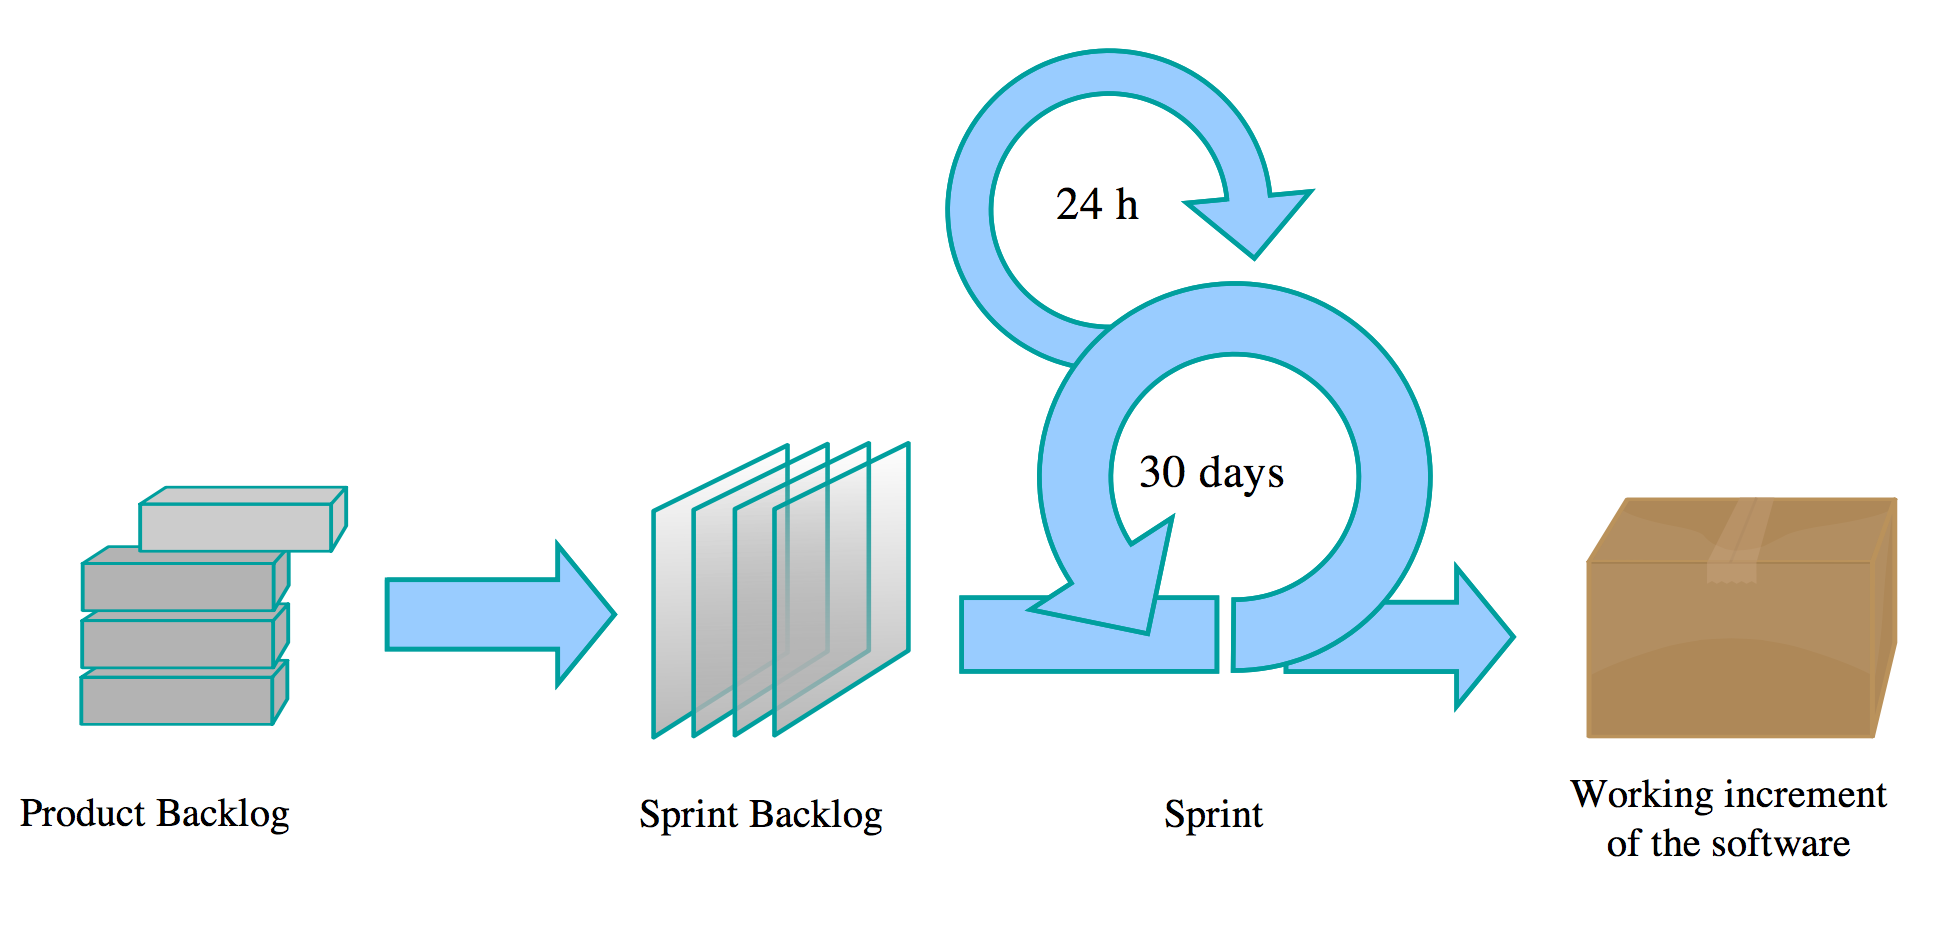
\includegraphics[width=150mm]{images/chapters/development_models/Scrum.png}
\caption{The Scrum cycle.}
\label{scrum}
\end{figure}

To end the section, as well as making a natural shift towards the next topic (Coordination), a look at Scrum-of-Scrums is carried out. It is a natural shift because Scrum-of-Scrums are used as the coordination mechanism across teams in the Scrum methodology. It works as the daily scrums (though usually implemented on a weekly basis because of time constraints and the complexity to find common times for all teams), but with one member assigned from each Scrum team to report completions, next steps and impediments for their respective teams. It is important that these impediments focus on the challenges that may impact coordination across teams and might limit other teams' work. The Scrum-of-Scrums will have their own backlog aiming to improve the cross-team coordination \cite{Sutherland2001}. Below the suggested questions for the SoS meetings are listed \cite{Cohn2007}:

\begin{enumerate}
  \item What did your team do since the previous meeting that is relevant to some other team?
  \item What will your team do by the next meeting that is relevant to other teams?
  \item What obstacles does your team have that affect other teams or require help from them?
  \item Are you about to put something in another team's way?
\end{enumerate}

Takeuchi et al. identified three strategies for distributed Scrum teams. The first type is isolated Scrum teams where teams operate as silos and no collaboration across teams is performed violating the agile principles. The second type is Scrum-of-Scrums which means overlapping Scrum teams. Here teams coordination, communicate and collaborate across teams through SoS meetings with participants from each team involved. Lastly, totally integrated Scrum teams are suggested. In this type teams are fully distributed and each team has members located at several sites. This approach creates similar characteristics as co-location. Type B is what is most common when several Scrum teams work together. The different types are visualised in figure \ref{distributedscrum} \cite{takeuchi2004}.

\begin{figure}
\centering
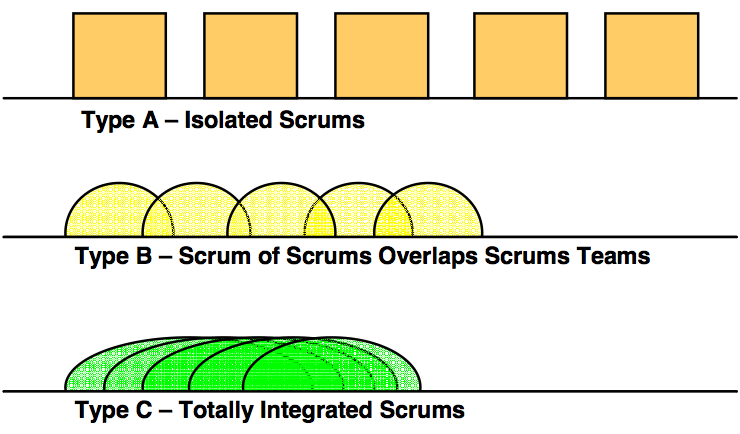
\includegraphics[width=110mm]{images/distributed_scrum.png}
\caption{Different strategies for distributed Scrum teams.}
\label{distributedscrum}
\end{figure}

\subsubsection{Kanban and Scrumban}
%Anderson

Kanban is a logistic control system that is closely related to lean software development. The word ``Kanban'' comes from two Japanese words: ``kan'' meaning visual and ``ban'' meaning board. The system was developed by Taiichi Ohno, an industrial engineer at Toyota. The reasoning behind developing this new system was to achieve and maintain a high level of production.

%http://link.springer.com/chapter/10.1007%2F978-3-642-20677-1_9
%Short description of Lean?

Cocco et al. described Kanban as the process of breaking down work to work items which are descriptions on cards (often post-it notes). These cards are then made visible for the entire team on a board. The board is used to show the flow of work within the team (or project). The high visibility comes from the cards and board showing which tasks are assigned to which member, communication priorities and highlights possible obstacles. An important feature of the Kanban method is to minimize Work in Progress (WIP) by reducing the amount of work items (cards) being developed at a time. This is done so the developers and customer can focus on smaller amounts, and should lead to an optimised process, as well as a reduced lead time. Compared to the Scrum methodology, Kanban (being a lean method) is able to release new futures more constantly, and not only at the end of each sprint iteration. Scrum is not able to change the requirements and direction of development in the middle of a sprint iteration, which Kanban can.

To get a more simplistic explanation of how the Kanban methodology works we can look at a standard work flow example. If a developer start on a task he moves this task from the ``work to be done'' section into the so-called ``work in progress'' column of the Kanban board. If there for some reason is a dependence towards other's work this particular work has to be moved to the ``on hold'' or ``waiting'' section of the board until the dependence is solved. After a task is completed it is moved into the final section of the board called the ``completed'' section. Teams also often use different colours to express the priority of the task, and tasks are often allocated to some specific part of the development, e.g., development, test etc. 

%TODO: Add kanban board?

%TODO: http://www.aboutscrumban.com/comparison-of-scrum-kanban-and-scrumban/
%TODO: http://www.aboutscrumban.com/

In later years a new approach has slowly surfaced which combines the Scrum and Kanban practices. This new methodology has been coined ``Scrumban'' (also referred to as ``Scrum-ban'' and ``Scrum ban''). The reasoning behind the evolution of this new methodology was that some practitioners felt that Scrum and Kanban did not fit all aspects of their work on their own with Scrum being too strict for constant change and releases (fast paced environments), and Kanban not being structured enough. The combination of the two methodologies is suppose to create a practice that fits a fast paced development environment. To get a better overview of the differences between Scrum, Kanban and Scrumban table \ref{coskas} is included.

\begin{center}
    \begin{longtable}{| p{2.6cm} | p{3.9cm} | p{3.9cm} | p{3.9cm} |}
   
    \hline & \textbf{Scrum} & \textbf{Kanban} & \textbf{Scrumban} \\ \hline
    \endfirsthead

    \multicolumn{4}{c}%
{{\bfseries \tablename\ \thetable{} -- continued from previous page}} \\ \hline
   & \textbf{Scrum} & \textbf{Kanban} & \textbf{Scrumban} \\ \hline
    \endhead

    \multicolumn{4}{|r|}{{Continued on the next page\ldots}} \\ \hline
    \endfoot

   \endlastfoot 

    \textbf{Iterations} & 1-4 week sprints & Continuous work alongside releases shorter than one week or bigger iterations like goals & Continuous work with short cycles for planning and longer cycles for release \\ \hline
    \textbf{Work routines} & Push and pull principle mixed with early binding to team members & Pull principle with late binding to team members & Pull principle with late binding to team members \\ \hline
    \textbf{Scope limits} & Sprint limits total work amount & Work in progress limits current work amount & Work in progress limits current work amount \\ \hline
    \textbf{Planning routines} & Sprint planning & Release/iteration planning, demand planning & Planning on demand for new tasks \\ \hline
    \textbf{Estimation} & Must be done before start of sprint & Optional & Optional \\ \hline
    \textbf{Performance metrics} & Burndown & Cumulative flow diagram, lead time cycle time & Average cycle time \\ \hline
    \textbf{Continuous improvement} & Sprint retrospective & Optional & Short Kaizen (continuous improvement) event as an option \\ \hline
    \textbf{Meetings} & Sprint planning, daily scrum, retrospective & Can be avoided & Short Kaizen event \\ \hline
    \textbf{Roles} & Product owner, Scrum master, team & Team and other work specific roles & Team and other work specific roles \\ \hline
    \textbf{Team members} & Cross-functional team members & Cross-functional team members, specialization is allowed & Specialization or preference to tasks \\ \hline
    \textbf{Task size} & The size that can be completed in sprint & Any size & Any size \\ \hline
    \textbf{New items in iteration} & Forbidden & Allowed whenever queue allows it & Allowed whenever queue allows it \\ \hline
    \textbf{Ownership} & Owned by a team & Supports multiple teams ownership & Supports multiple teams ownership \\ \hline
    \textbf{Board} & Defined/reset each sprint & Persistent & Persistent \\ \hline
    \textbf{Prioritization} & Through backlog & Optional & Recommended on each planning \\ \hline
    \textbf{Roles} & Scrum master, product owner, team & Not defined, may vary & Not defined, may vary \\ \hline
    \textbf{Rules} & Constrained process & Only a few constraints, flexible process & Slightly constrained process \\ \hline
    \textbf{Fit for} & Enterprise maturity for teams working on product or especially project which is longer than a year & Support and maintenance teams, continuous product manufacturing & Startups, fast-pace projects, continuous product manufacturing \\ \hline 

    \caption{Comparison of Scrum, Kanban and Scrumban}
    \label{coskas}
    \end{longtable}
\end{center}

%CEEOL (lasted ned artikkel)
%http://leansoftwareengineering.com/ksse/scrum-ban/
%http://en.wikipedia.org/wiki/Scrum_ban

\subsubsection{Pair programming}

Pair programming is a common practice in software development where two developers work side-by-side on the same computer, continuously collaborating and communicating on the same code. The thought behind the practice is to realise several potential benefits, such as:

%http://collaboration.csc.ncsu.edu/laurie/Papers/XPSardinia.PDF
%http://cacm.acm.org/magazines/2000/5/7671-all-i-really-need-to-know-about-pair-programming-i-learned-in-kindergarten/fulltext
%http://citeseerx.ist.psu.edu/viewdoc/download?doi=10.1.1.258.7427&rep=rep1&type=pdf

\begin{itemize}
  \item Production speed is faster in the long-term, and the pair comes up with a larger amount of possible solution than two developers working individually. This is called the ``pair programming advantage''.
  \item Code and general design quality is a lot higher (few bugs and defects). This is called the ``pair defect advantage''.
  \item Better job-satisfaction working in pairs than alone.
  \item Pair programming increases learning as knowledge is constantly shared between the two programmers.
  \item As developers are so tightly coupled in pair programming the team-building and communication improves.
\end{itemize}

There are three possible types of pairings in pair programming. These are explained below with their potential benefits and drawbacks:

\begin{itemize}
%http://www.sciencedirect.com/science/article/pii/S1071581906000644
  \item \textbf{Senior-Senior:} With two experts conducting the pair programming together this would in theory be the most productive pairing leading to the best results, however, such a pairing has shown to often cause problems as the seniors are less likely to question established practices.
%Williams, L. and Kessler, R. (2003). Pair Programming Illuminated. Boston: Addison-Wesley Professional.
  \item \textbf{Senior-Junior:} With a combination of both a senior and a junior developer often new ideas and solution surface as the junior programmer is more likely to question established practices, also leading to senior developers having to think through these practices. It is however important that the junior developer does not take an observer role, but is involved in the coding with the expert.
%http://collaboration.csc.ncsu.edu/laurie/Papers/XPSardinia.PDF
  \item \textbf{Junior-Junior:} The last pairing has two novice developers collaborating. Results have shown that two junior programmers working together yield better results than the two developers working separately, and is often used in academic settings.
\end{itemize}

\section{Coordination}

This section takes a look at different publications on coordination. It starts of with Malone and Crowston's well-known coordination theory. After this has been described a closer look at Strode's theoretical model of coordination is outlined. Ending the chapter is a brief look at the complexity factor introduced with a large-scale context in coordination.

\subsection{Malone and Crowston's Coordination Theory}

One of the most well-known papers on coordination theory was published by Malone and Crowston in 1990 and further redefined in 1994 (the focus will be on this paper) \cite{Malone1994}. Their study spanned different fields and can therefore be seen as an interdisciplinary coordination study. They listed an extensive amount of different definitions of coordination, and through these proposed definitions come up with a rather simple definition:

\begin{fancyquotes}
Coordination is managing dependencies between activities.
\end{fancyquotes}

These dependencies can occur when some task has to be postponed or extended because of its connection to another task, resource or unit. Their theory is based on a combination of coordination from several different disciplines such as computer science, organization theory, operations research, economics, linguistics, and psychology. They state that coordination consists of one or more coordination mechanisms, and that each of these address one or more dependencies.

While Strode et al. acknowledges their coordination theory as very useful for identifying these so-called dependencies, categorising them, and identifying coordination mechanisms in a situation, they conclude that it is only a theory for analysis and not intended to be used for prediction. Despite this being true, and the coordination theory not being suitable for predicting outcomes such as coordination effectiveness, their theory adds important information for better understanding of how activities or artefacts support coordination in organisational settings \cite{Strode2012}.

\subsection{Mintzberg's Coordination Mechanisms}

%TODO: Mintzberg, H.: Mintzberg on Management: Inside Our Strange World of Organizations (1989)

Around the 1980s Mintzberg performed well-known studies on organisational structures focusing on the division of labour into tasks to be carried out, and the coordination of these tasks to complete the activity. With this research six coordination mechanisms were identified in which organisations can coordinate their work:

\begin{itemize}
  \item In \textbf{direct supervision} there is typically one person, e.g., a manager, giving orders to other members and with that coordinating their work.
  \item In the \textbf{standardisation of work processes} coordination of the work happens through standards such as guidelines, orders, rules and regulations.
  \item In the \textbf{standardisation of outputs} the work is coordinated by performance standard measures of the outputs of the work.
  \item In the \textbf{standardisation of skills} coordination happens through standardisation of skills and knowledge, typically before the personnel starts performing the work.
  \item In the \textbf{standardisation of norms} it is the norms that are used to coordinate, meaning all members operate according to the same beliefs.
  \item In \textbf{mutual adjustment} the members coordinate their own work by informal communication with each other.
\end{itemize}

For agile software development it is in particular the mutual adjustment mechanism that is present. Because of its nature it is well suited for complex, dynamic and innovative environments. With the large focus on rapid and continuous delivery the use of informal communication arenas are to a great degree existent in agile software development.

\subsection{Strode's Theoretical Model of Coordination}
\label{strodechap}

Strode et al. performed a multi-case study on three different co-located agile projects in 2012 \cite{Strode2012}. From these projects the findings led to a theoretical model of coordination that will be outlined in this section. It is important to note that these projects were not large-scale, but the model will nonetheless be used to compare if there are similarities from the model proposed by Strode et al., and the findings from the literature review on large-scale agile project coordination. This will be performed in chapter \ref{results}, \ref{disc} and \ref{concl}.

From these case studies three main components for the theoretical model were extracted: Synchronisation, Structure and Boundary Spanning. These components combine to what is called the ``Coordination Strategy''. Coordination strategy is in this context a group of coordination mechanisms that manage dependencies in a situation. The theoretical model of coordination can be seen in figure \ref{strode}. Below the three main components will be explained in more detail:

\begin{figure}
\centering
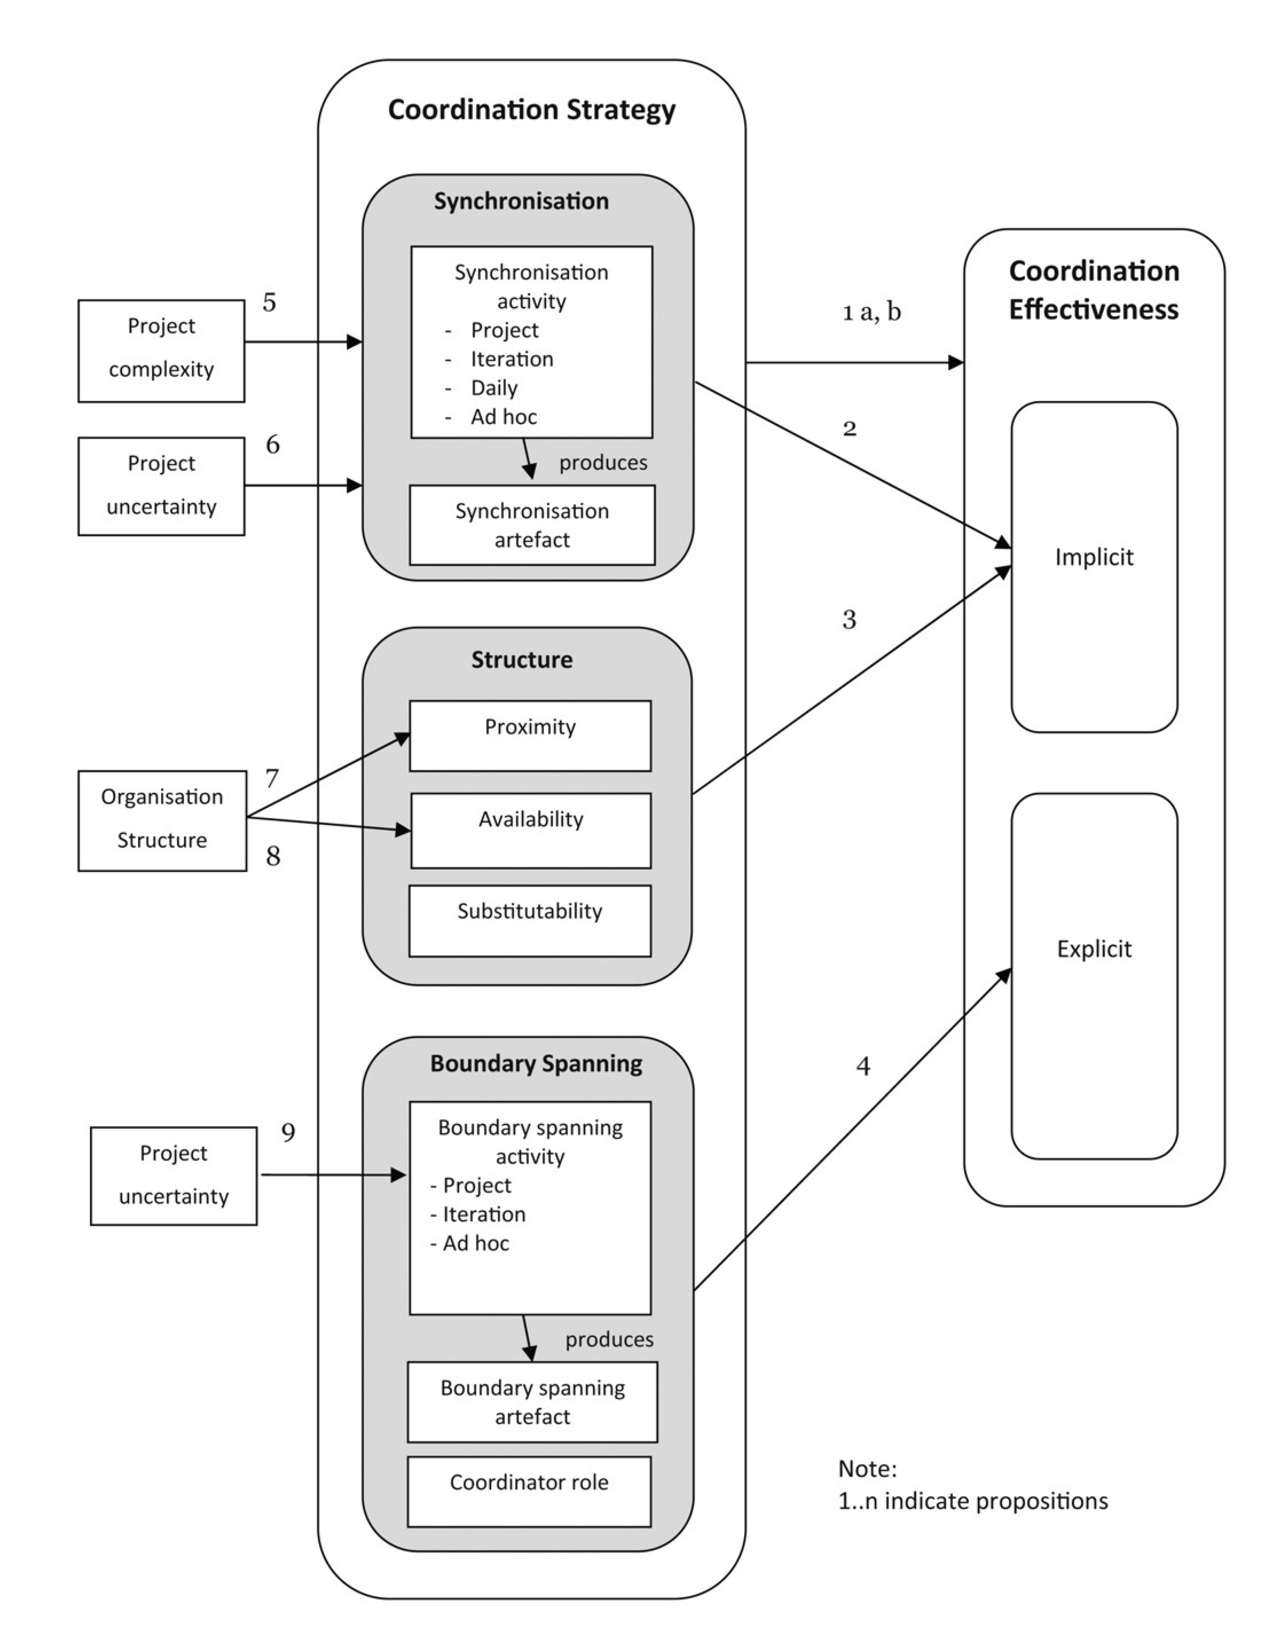
\includegraphics[width=160mm]{images/Strode.pdf}
\caption{A theory of coordination in agile software development projects.}
\label{strode}
\end{figure}

\subsubsection{Synchronisation}

Synchronisation in this context consists of synchronisation activities and synchronisation artefacts produced and used during these activities. Synchronisation activities are activities performed by all team members simultaneously. They contribute to a common understanding of the task, process, and or expertise of other team members. Synchronisation artefacts on the other hand are artefacts that are generated during synchronisation activities. These artefacts may be visible for the entire team or largely invisible but available. The artefacts can take a physical or virtual form, and are temporary or permanent.

\subsubsection{Structure}

Structure in this model is the arrangement of, and relations between, the parts of something complex. It consists of three categories: proximity, availability and substitutability. Proximity is the physical closeness of other (individual) team members. Availability means that other team members are accessible for requests or information. Lastly, substitutability has to do with the team members ability to perform others' work to maintain time schedules.

\subsubsection{Boundary Spanning}

The last component of the coordination strategy is boundary spanning. Boundary spanning has to do with the interaction with other organisations or other business units that are not involved in the project. It consists of three aspects: boundary spanning activities, boundary spanning artefacts and a coordinator role. Boundary spanning activities are activities performed to achieve help from some unit or organisation not involved in the project. The boundary spanning artefacts are artefacts produced to enable this external coordination. These artefacts have the same characteristics as synchronisation artefacts. Lastly, the coordinator role is a role taken by someone within the project team. His or her role is to support interaction to outside personnel to extract resources or information needed in the project at hand.

\subsubsection{Coordination Effectiveness}

There is another important part of the theoretical model of coordination, namely the coordination effectiveness concept. This concept will be further explained in section \ref{efficiency} that takes a look at coordination effectiveness.

\subsubsection{Propositions}

There are in total ten propositions (Proposition 1 has two parts) linking the coordination concepts in Strode's theoretical coordination model showed in figure \ref{strode}. These are outlined below:

\begin{fancyquotes}
\textbf{Proposition 1a:} A coordination strategy that includes synchronisation and structure coordination mechanisms improves project coordination effectiveness when the customer is included in the project team. Synchronisation activities and associated artefacts are required at all frequencies – project, iteration, daily, and ad hoc.
\end{fancyquotes}

\begin{fancyquotes}
\textbf{Proposition 1b:} A coordination strategy that includes synchronisation, structure, and boundary spanning coordination mechanisms improves project coordination effectiveness when the customer is an external party to the project. Synchronisation activities and associated artefacts are required at all frequencies – project, iteration, daily, and ad hoc. Boundary spanning activities and associated artefacts are required at all frequencies – project, iteration, and ad hoc.
\end{fancyquotes}

\begin{fancyquotes}
\textbf{Proposition 2:} Synchronisation activities at all frequencies – project, iteration, daily, and ad hoc, along with their associated synchronisation artefacts, increase implicit coordination effectiveness.
\end{fancyquotes}

\begin{fancyquotes}
\textbf{Proposition 3:} Structural coordination mechanisms i.e. close proximity, high availability, and high substitutability, increase implicit coordination effectiveness.
\end{fancyquotes}

\begin{fancyquotes}
\textbf{Proposition 4:} High levels of boundary spanning coordination mechanisms, i.e. boundary spanning activities at all frequencies – project, iteration, and ad hoc, their associated boundary spanning artefacts, and a coordinator role, increases explicit coordination effectiveness.
\end{fancyquotes}

\begin{fancyquotes}
\textbf{Proposition 5:} Under conditions of high project complexity, increasing the frequency of iteration and ad hoc synchronisation activities will maintain coordination effectiveness. The production of related synchronisation artefacts must be adjusted accordingly.
\end{fancyquotes}

\begin{fancyquotes}
\textbf{Proposition 6:} Under conditions of high project uncertainty, to maintain synchronisation activity frequency and production of associated artefacts, changing the priority of stories will maintain coordination effectiveness.
\end{fancyquotes}

\begin{fancyquotes}
\textbf{Proposition 7:} A mono-project organisation structure enables close proximity relative to multi- or matrix structures.
\end{fancyquotes}

\begin{fancyquotes}
\textbf{Proposition 8:} A mono-project organisation structure improves availability relative to multi- or matrix style structures.
\end{fancyquotes}

\begin{fancyquotes}
\textbf{Proposition 9:} Under conditions of high project uncertainty, when the customer is not part of the team, increased boundary spanning coordination mechanisms will maintain coordination effectiveness. The production of related boundary spanning artefacts must be adjusted accordingly.
\end{fancyquotes}

\subsection{Coordination in Large-scale}
\label{largescalecor}

This section takes a closer look at general studies performed on large-scale coordination and is not specifically focusing on software development. The section is added to highlight the introduction of complexity that a large-scale context brings with it.

Van der Ven et al. released an article in 1976 where they tried to identify determinants of coordination modes within organisations. They state that an increase in size will produce a trade-off between the increasing complexity and cost of coordination at the administrative level. From the research two different coordination forms are described, namely vertical and horizontal. The vertical communication includes coordination through curators, while the horizontal communication occurs by way of one-to-one communication. Their findings show that when team size increases the coordination moves towards a more vertical and impersonal style \cite{Ven1976}. This is backed up by John Child in a publication from 1973. Here he states that with a growing complexity level there is likely that administrative problems will occur regarding coordination and control \cite{Child1973}.

\section{Large-scale}

Having looked at coordination in large-scale in section \ref{largescalecor}, what is actually this so-called ``large-scale''? This was a topic brought up at a workshop regarding research challenges in large-scale agile software development where opinions regarding how large-scale should be defined varied a lot. Some suggestions were to define it through project duration, project cost, number of people involved, number of remote sites and/or number of teams \cite{Dingsoyr2013b}. This issue was further analysed by Dingsøyr, Fægri and Itkonen trying to work out a taxonomy of scale for agile software development. Their results are summarised in table \ref{Scale} where the taxonomy of scale is based on the amount of teams involved in the development project \cite{Dingsoyr2013a}.

\begin{table}
\begin{center}
    \begin{tabular}{| l | l | p{7cm} |}
    \hline
    \textbf{Level} & \textbf{Number of teams} & \textbf{Coordination approaches} \\ \hline
    Small-scale & 1 & Coordinating the team can be done using agile practices such as daily meetings, common planning, review and retrospective meetings. \\ \hline
    Large-scale & 2-9 & Coordination of teams can be achieved in a new forum such as a Scrum of Scrums forum. \\ \hline
    Very large-scale & 10+ & Several forums are needed for coordination, such as multiple Scrum of Scrums. \\
    \hline
    \end{tabular}
    \caption{A taxonomy of scale of agile software development projects.}
    \label{Scale}
\end{center}
\end{table}

Others have also discussed problems regarding large-scale. For example Schnitter and Mackert discuss the scaling of Scrum at SAP AG and concludes that in their case the maximum involved development employees that may be organised with regards to agile project management is 130 (This number sums up developers in 7 teams (max. 70 people), the product team (max. 16), development infrastructure responsible (about 10), quality assurance and testers (about 25), general management (about 10)) \cite{Nord2011}.

Another example is taken from Nord et al. defining large-scale by scope of the system, team size, and project duration. They say that the size of the development team must be more than 18 people and distributed into a few teams \cite{Robert2014}.

So the definition of a ``large-scale agile project'' used in this research will be:

\begin{fancyquotes}
An agile project must consist of a minimum amount of two teams coordinating across the teams to be categorised as large-scale.
\end{fancyquotes}

\textbf{ }

\section{Multiteam Systems}
%TODO: Ha med referanse til tidligere?
%TODO: Cites i avsnitt
As mentioned earlier the work environments have become more challenging and complex in line with the growth of communication and information technology. This growth has led to the globalisation of organisational work. With the globalisation an increase in interconnectivity across organisational boundaries has become apparent. Because of this trend new questions and problems have surfaced. Unfortunately, these questions and problems have not been possible to adapt to traditional organisational forms. This has led to the introduction of new and different organisational forms, e.g., matrix and virtual organisations, and cross-functioning and ad hoc project teams. One of these new organisational forms focus on projects where collaboration exists across traditional team and organisational boundaries. This form does not resemble traditional organisations or large-scale teams, but can be seen as an aggregation that includes tightly coupled arrangement of teams, where the different teams may have noticeable different norms, expertise, missions, structures and operating procedures to the overall work. Mathieu, Marks, and Zaccaro \cite{TODO} defined the organisations corresponding to the aforementioned form as multiteam systems (MTSs). Below their definition follows:

\begin{fancyquotes}
Two or more teams that interface directly and interdependently in response to environmental contingencies towards the accomplishment of collective goals. MTS boundaries are defined by virtue of the fact that all teams within the system, while pursuing different proximal goals, share at least one common distal goal; and in doing so exhibit input, process and outcome inter-dependence with at least one other team in the system \cite{TODO}.
\end{fancyquotes}

From this definition it is easy to see similarities with so-called ``large-scale'' projects and organisations. Both large-scale projects' and multiteam systems' taxonomies look at the amount of teams involved, where the minimum number is two, but are typically larger than this number by a considerable margin. In both categories the teams have to be somewhat interconnected, and the organisational boundaries may be crossed, meaning teams can reside in different organisations. Mathieu et al. have therefore categorised MTSs into ``internal MTSs'' where the whole system or project is situated within an organisation, and ``cross-boundary MTSs'' where teams are located in different organisations, hence organisational boundaries have to be crossed to achieve collaboration \cite{TODO}.

One of the most distinguishing factors of multiteam systems is their focus on goal hierarchies. As mentioned above interdependencies are not only witnessed within teams, but also across them. From the definition of MTSs the teams have different proximal goals, but all share at least one distal goal. Mathieu et al. define the feature of these goal hierarchies that are relatively common across different MTSs as:

\begin{enumerate}
  \item MTS goal hierarchies have a minimum of two levels
  \item Goals at higher levels entail greater interdependent actions among more component teams than goals at lower levels
  \item The superordinate goal at the apex of the hierarchy rests on the accomplishment by component teams of all lower order goals
  \item Higher order goals are likely to have a longer time horizon than lower order goals
  \item Goals vary in their priority and valence
\end{enumerate}

%TODO: Skrive om ulike typer interdependencies?

\subsection{MTS Characteristics}

Having looked at the features of multiteam systems the attention is shifted towards their attributes. These attributes are what separates different MTSs. The attributes are classified into three dimensions, compositional, linkage and development attributes, and will be presented in the following sections. The different dimensions are summarised in table \ref{domsc}.

\subsubsection{Compositional Attributes}

In the compositional dimension several demographic features of the MTS and characteristics of component teams are looked at. In total there are ten attributes, and these will be outlined in this section. Regarding the magnitude of the MTSs two attributes are used. Firstly the ``number'' of component teams located within the MTS, and secondly the total ``size'' of the MTS, meaning the amount of individual members involved in the multiteam system.

%Skrive om problemer som kan oppstå når det blir for mange team/medlemmer?

Another compositional attribute that was earlier mentioned as a distinguishing factor is ``boundary spanning''. This attribute is concerned with where the different component teams originate from. If all component teams come from the same organisation it is an internal MTS, while if the component teams come from two or more organisations it is an external MTS. External MTSs are more complex and are more likely to run into task and social complexity than its counterpart. In this context, social complexity refers to diversity, scale, scope, and dynamism of stakeholders in the MTS's environment \cite{?}. There are two more attributes concerned with boundary spanning which are at a higher detail level. Firstly the ``organisational diversity'' looks at the total amount of organisations represented in the MTS. With a higher number of organisations the likelihood of a higher level of social complexity rises. Secondly the ``proportional membership'' outlines the percentage of teams from different organisations. With an unbalanced proportional membership there is a risk that the influence level will be greater from the organisation(s) with the highest amount of teams.

%TODO: Usikker på om det er i teams eller mellom teams det er snakk om?
The sixth compositional attribute is concerned with how similar the different component teams' core task and goals are. This attribute is called ``functional diversity''. With an increase in this so-called functional diversity problems may occur. Another important factor in MTSs is ``geographic dispersion''. There are three degrees of geographical dispersion, namely co-located, partially co-located, and fully dispersed. Some problems that have been witnessed in dispersed projects has been communication issues, coordination difficulties and trust building. Building on the geographic dispersion is an attribute called ``cultural diversity''. If teams are dispersed and the boundaries extend the national borderline this could lead to cultural clashes.

The ninth attribute in the compositional dimension is ``motive structure''. This attribute refers to the degree to which the different teams commit to the MTS, and how compatible and closely linked the team goals and the MTS goals are. A problem that can occur in this compositional attribute is that a team's proximal and/or distal goals are in conflict with the overall goals of the MTS leading to more complex interteam processes. With an increase in incompatibility in goals between the MTS and the compositional team(s) this can lead to team members being less committed to the overall goal hierarchy of the multiteam system. Motive structure may be associated with the last compositional attribute called ``temporal orientation''. Temporal orientation is concerned with the amount of resources dedicated to the MTS by each component team.

As can be seen the compositional attributes are important factors in interteam dynamics within MTSs. Focus on team composition is important to keep the level of effectiveness high, as well as prohibiting evolution of subgroups.

\subsubsection{Linkage Attributes}

Moving on the focus is shifted towards the so-called linkage dimension. Linkage mechanisms and attributes are concerned with how teams are arranged and connected within a multiteam system. The first attribute is concerned with the amount of coordination between different component teams that is needed and is called ``interdependence''. The degree of interdependence will differ from different MTSs, but with an increasing interdependence the amount of interteam processes necessary will increase to achieve high MTS effectiveness.

Two other linkage attributes that often correlate are ``hierarchical arrangement'' and ``power distribution''. Hierarchical arrangement focuses on how teams are organised within the MTS with regards to their responsibility level of goal attainment. The more proximal goals the component team is involved with, the higher in the hierarchical arrangement they are. As for power distribution the focus is on the relative influence that component teams have within a multiteam system. Often the teams placed higher in the hierarchical arrangment, meaning they have more proximal goals, also have a bigger influence and power. Other factors that could lead to higher power can be team size, the team's functional centrality to the core mission of the MTS, and/or the parent organisations having assigned the team with authority. Both attributes will likely influence communication, interaction and collaboration between the component teams in a multiteam system.

Moving on to the forth and fifth linkage attributes the focus is shifted towards the communication structures of MTSs. Firstly ``communication networks'' refer to the most common interaction and communication patterns between and within component teams. These networks can be fully decentralised (everyone interactive with everyone), fully centralised (everyone communicate to and through one single member of the MTS), and various patterns between these two boundary points. It is important to notice that the chosen communication network in a multiteam system will have a great impact on the task efficiency of the MTS. Lastly ``communication modality'' is concerned with which modes are used to communicate across component teams within a multiteam system. These can be, e.g., face-to-face interaction, electronic communication, or a mixture of the two. Often the degree of which modes are used is closely linked to the aforementioned compositional attribute called ``geographic dispersion''. With co-located teams preferring a higher amount of face-to-face communication.

\subsubsection{Developmental Attributes}

The last dimension of multiteam systems is the developmental. Developmental attributes are concerned with the developmental dynamics and patterns of MTSs. The first attribute looks at how the MTS was put to life, its ``genesis''. The origin of MTSs can either occur through appointment from parent organisations, or they may emerge from collective initiative of several teams. The type of genesis can have an impact on different aspects of a MTS, e.g., the distal goal. Another developmental attribute is ``direction of development'' and looks at the direction the MTS takes from its origin. For example the MTS could have emerged from a specific event, but then move towards a more formalised entity as time passes. Another development path could be the MTS being formally planned in anticipation of a possible situation occurring, but when the event does occur acctually evolve in membership and linkages.

Two other developmental attributes are ``tenure'' and ``stage''. The tenure attribute is concerned with the anticipated  duration of the MTS, while the stage attribute looks at which particular stage of development the MTS is in. Starting as a newly formed multiteam system it will evolve through different phases to finally becoming a mature MTS. The stage of MTS development will often give a hint to the efficiency of the MTS's interteam processes. 

%Skrive mer om hva som skjer når nye team kommer inn? Skrive mer om "adaptation"?
The last two developmental attributes together combine to the group term ``transformation of system composition'', meaning if there are changes to the composition as the MTSs develop and move through the different phases of development. The first of these focuses on ``membership constancy'' and refers to how constant or fluid the number of component teams are. Often in more complex and turbulent environments the amount of component teams may change over the course of the MTS's lifespan. Lastly ``linkage constancy'' is concerned with how the component teams are connected. The focus is on if these linkages between the component teams in a multiteam system is constant or if they change as the MTS progresses. Again the likelihood of fluidity in coordination structures between teams is higher when the MTS is located in more turbulent and dynamic environments.

In the above sections three dimensions of multiteam systems and their attributes have been presented. It is important to note how the different attributes can be factors in achieving effective MTSs and MTS processes. A simple model of MTS effectiveness is outlined in figure \ref{amomse}, where the attributes of the compositional, linkage and developmental dimensions can be seen as predecessors of different intrateam and interteam processes. The effects of these attributes on the total effectiveness of the multiteam system would be arbitrated by these intra- and interteam processes.

\begin{figure}
\centering
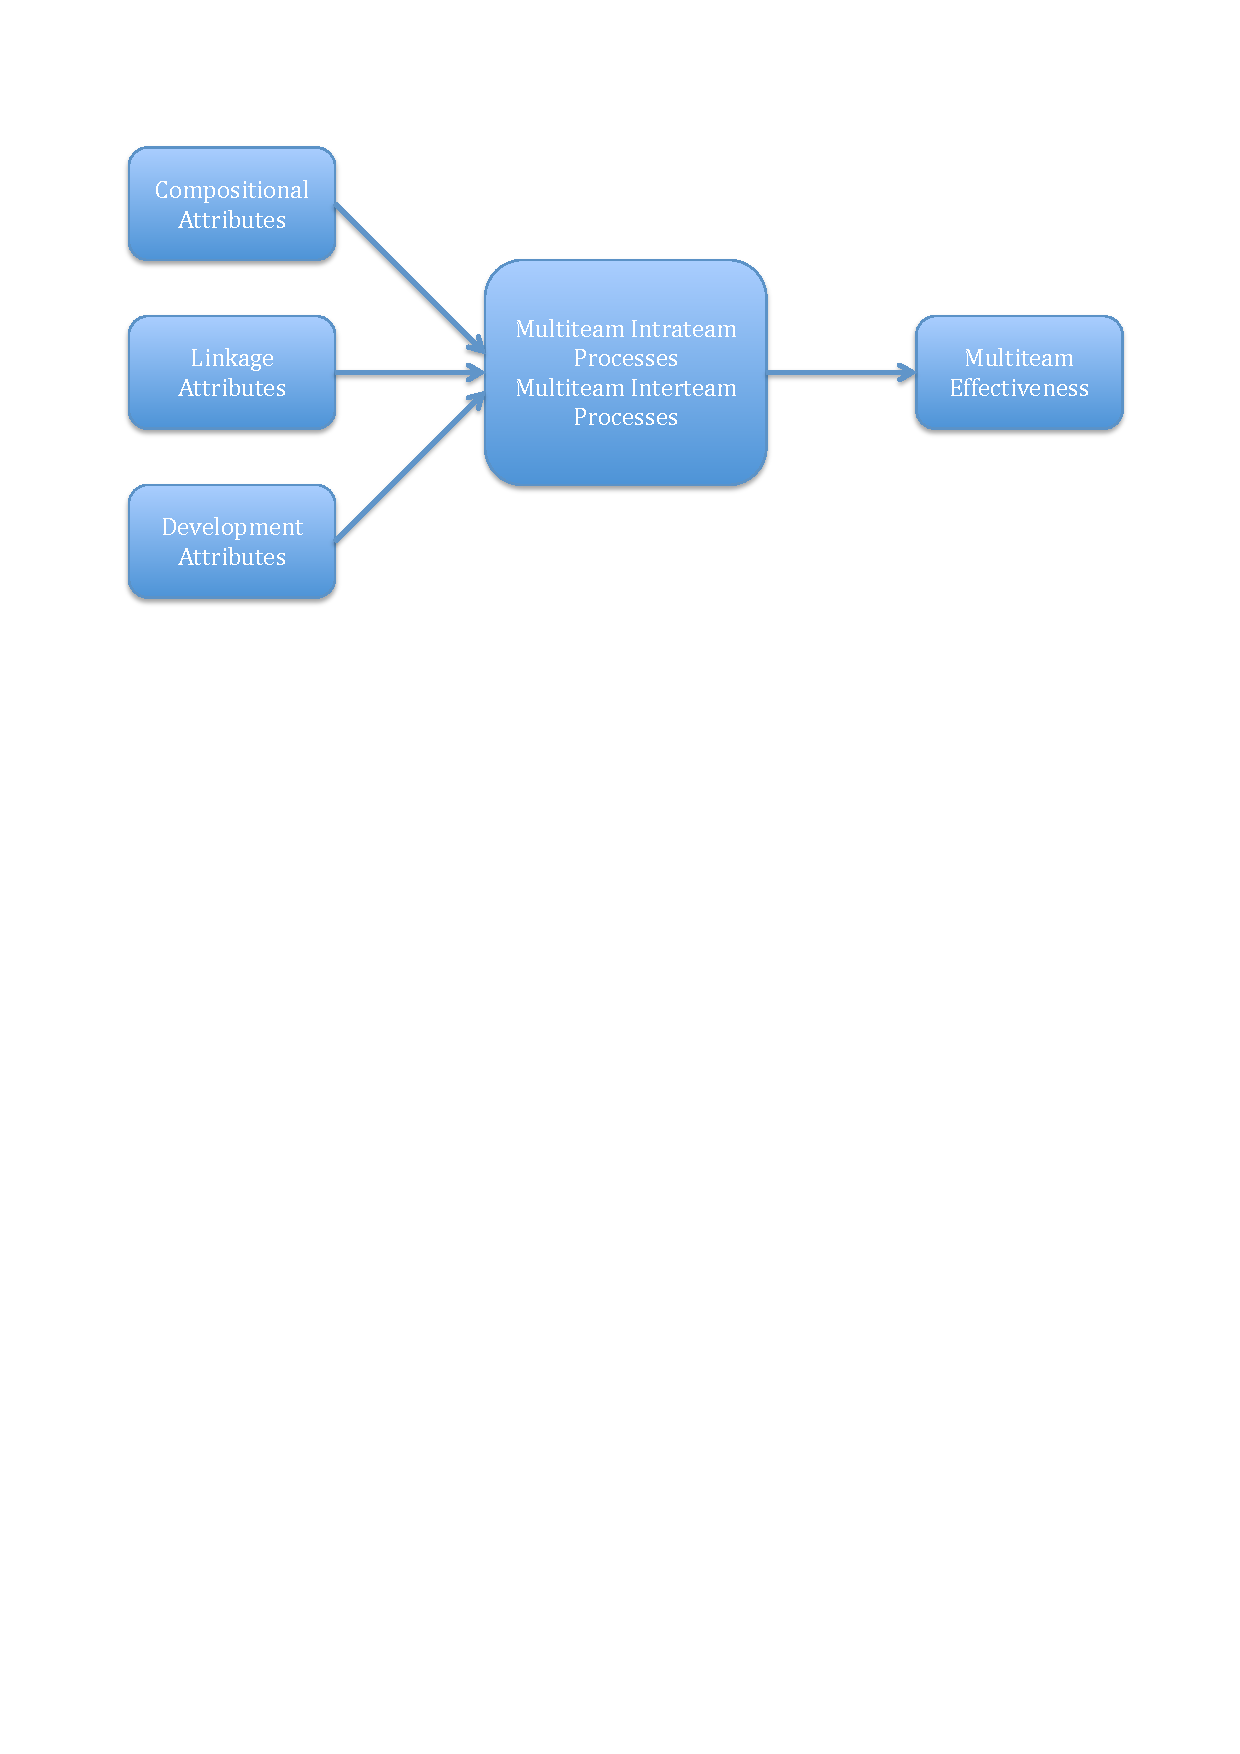
\includegraphics[trim = 15mm 190mm 15mm 10mm, width=150mm]{images/multiteam_system_model.pdf}
\caption{A model of multiteam system effectiveness.}
\label{amomse}
\end{figure}


%TODO: Fiks tabell
\begin{center}
\begin{longtable}{ | p{2.5cm} | p{4cm} | p{8cm} | }

   
    \hline \textbf{Dimension} & \textbf{Attribute} & \textbf{Explanation} \\ \hline
    \endfirsthead

    \multicolumn{3}{c}%
{{\bfseries \tablename\ \thetable{} -- continued from previous page}} \\ \hline
   \textbf{Dimension} & \textbf{Attribute} & \textbf{Explanation} \\ \hline
    \endhead

    \multicolumn{3}{|r|}{{Continued on the next page\ldots}} \\ \hline
    \endfoot

   \endlastfoot 

	\multirow{10}{*}{Compositional} & Number & Number of component teams within the MTS \\ \cline{2-3}
 	& Size & Total number of individual members across teams \\ \cline{2-3}
 	& Boundary status & Component teams come from single organization (internal) versus multiple organisations (external or cross-boundary) \\ \cline{2-3}
 	& Organisational diversity & In a cross-boundary MTS, the number of different organisations represented among the component teams \\ \cline{2-3}
	& Proportional membership & In a cross-boundary MTS, the percentage of teams from different organisations \\ \cline{2-3}
	& Functional diversity & Degree of heterogeneity in the core purposes and missions of component teams \\ \cline{2-3}
	& Geographic dispersion & Co-located or dispersed component teams \\ \cline{2-3}
	& Cultural diversity & Degree to which component teams come from different nations or cultures \\ \cline{2-3}
	& Motive structure & Degree of commitment of each component team to the MTS; the compatibility of team goals and MTS goals \\ \cline{2-3}
	& Temporal orientation & Level of effort and temporal resources expected of each component team \\ \cline{2-3}
\hline
	\multirow{5}{*}{Linkage} & Interdependence & Degree of integrated coordination (e.g., input, process, outcome) among members of different component teams \\ \cline{2-3}
 	& Hierarchical arrangement & Ordering of teams according to levels of responsibility \\ \cline{2-3}
 	& Power distribution & The relative influence of teams within the MTS \\ \cline{2-3}
	& Communication structure: Network & The typical patterns of interteam communication \\ \cline{2-3}
	& Communication structure: Modality & The modes of communication (e.g., electronic, face-to-face, or mixed) that occur across component teams \\ \cline{2-3}
\hline
	\multirow{6}{*}{Developmental} & Genesis & The initial formation of an MTS as either appointed or emergent \\ \cline{2-3}
 	& Direction of development & From emergent to formalised; an evolution from an early formal state \\ \cline{2-3}
	& Tenure & The anticipated duration of the MTS \\ \cline{2-3}
	& Stage & The stage of MTS development from newly formed to mature \\ \cline{2-3}
	& Transformation of system composition: Membership constancy & Fluidity versus constancy of component teams as members \\ \cline{2-3}
	& Transformation of system composition: Linkage constancy & Fluidity versus constancy of linkages among component teams \\ \cline{2-3}
	\hline
\caption{Dimensions of multiteam system (MTS) characteristics.}
\label{domsc}
\end{longtable}
\end{center}

\section{Efficiency, Effectiveness, Productivity and Performance in Coordination}
\label{efficiency}

There has been released a good amount of papers regarding effectiveness, productivity and efficiency in project literature. Unfortunately research in this area that focuses on large-scale is scarce. Therefore, the work highlighted in this section will mainly be extracted from small-scale studies. To start the section of a closer look at the aforementioned study by Strode et al. will be performed, before a summary of some different field studies on the matter will be carried out.

\subsection{Strode's Coordination Effectiveness}
\label{cordinationeffectiveness}

Part of the theoretical model of coordination by Strode et al. seen in figure \ref{strode} is the so-called ``coordination effectiveness''. This concept was developed by Strode et al. in 2011 having used the same three agile projects discussed earlier, as well as a non-agile software development project as a foundation \cite{Strode2011}. Coordination effectiveness is defined as the outcome of a particular coordination strategy. Coordination effectiveness is split into two components: an implicit and an explicit part.

The implicit part is concerned with coordination that occurs without explicit speech or message passing, this happens within work groups. It has five components: ``Know why'', ``Know what is going on and when'', ``Know what to do and when'', ``Know who is doing what'', and ``Know who knows what''. These aspects are pretty self-explanatory.

The explicit component on the other hand is concerned with the physical aspects of the project. It states that the objects involved in the project have to be in the correct place, at the correct time and in a state of readiness for use. A summary of the combination of explicit and implicit coordination effectiveness is provided in figure \ref{effectiveness}.

\begin{figure}
\centering
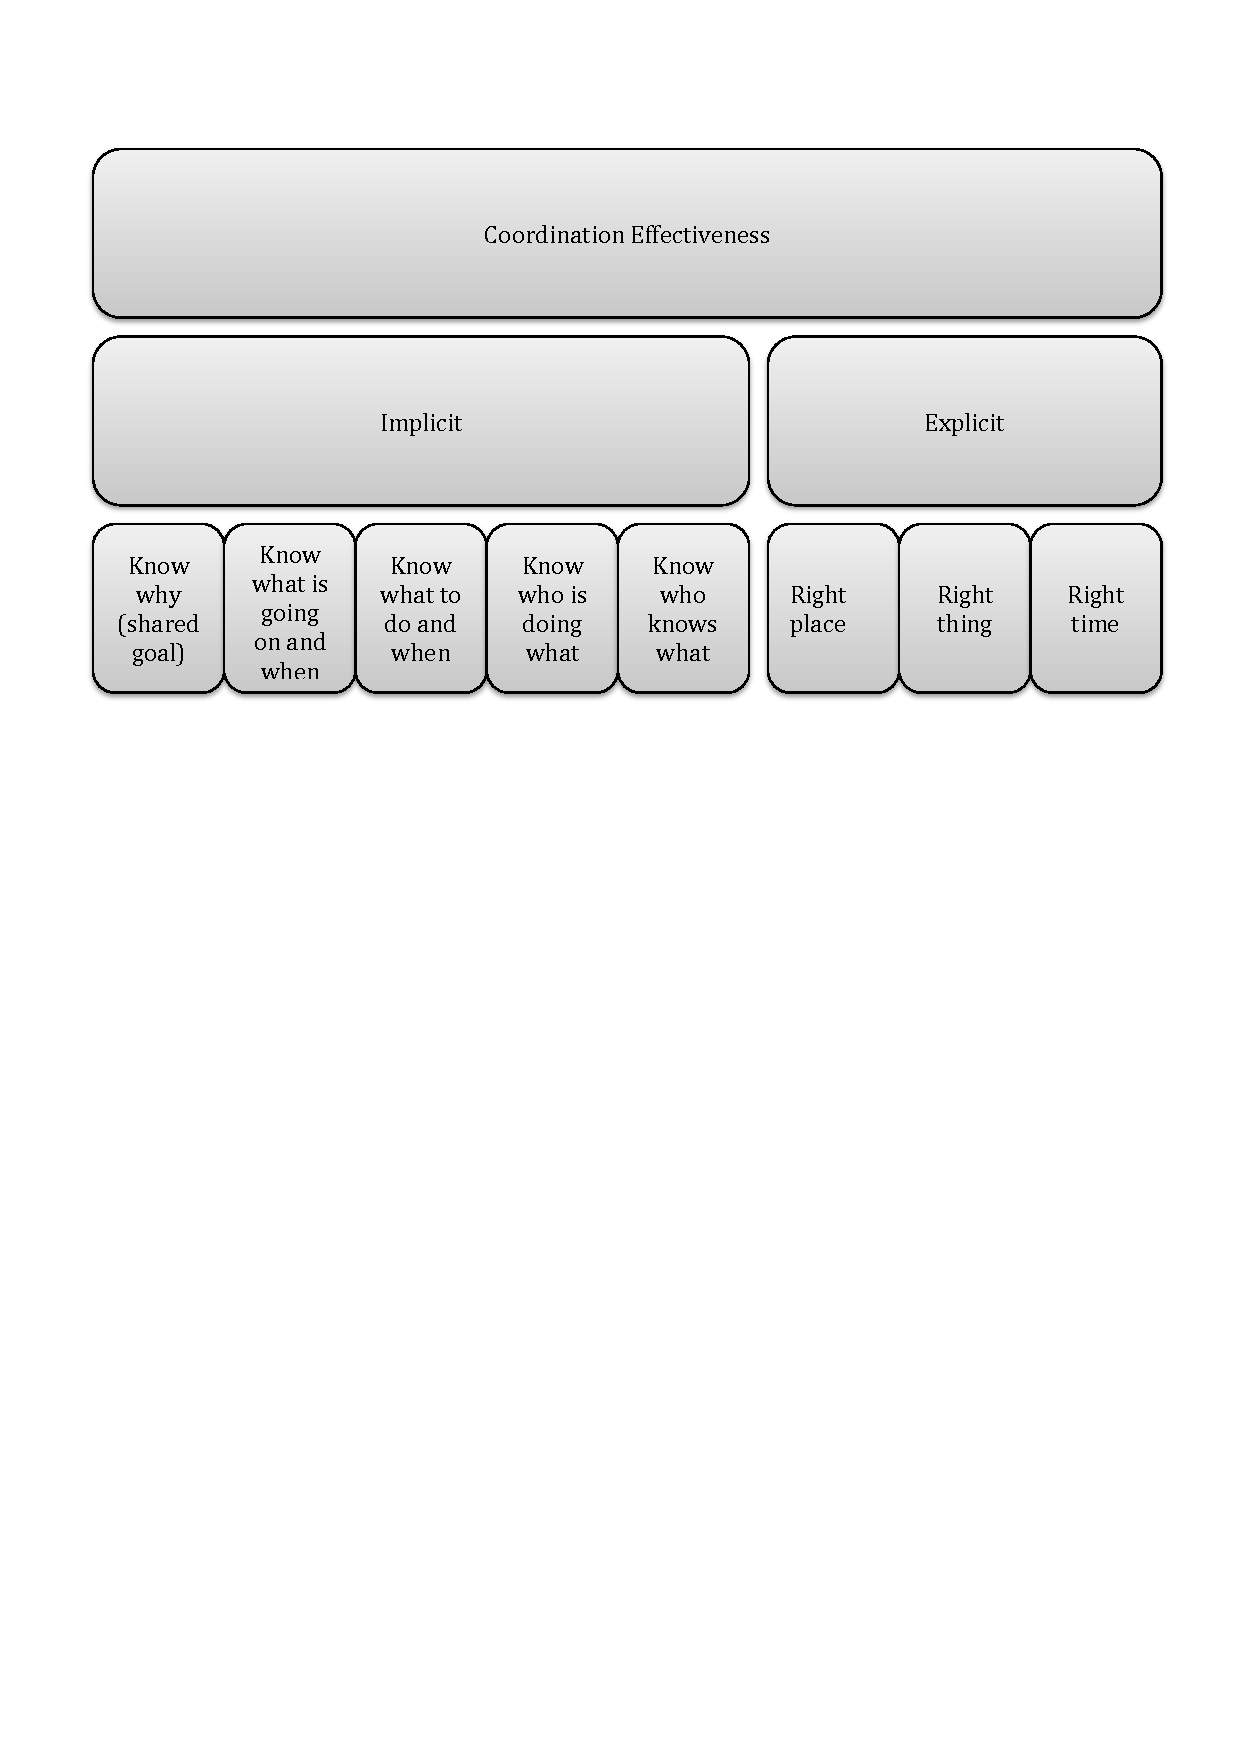
\includegraphics[trim=0cm 17.5cm 0cm 1.5cm, width=160mm]{images/Coordination_Effectiveness.pdf}
\caption{Components of coordination effectiveness from Strode et al. (2011).}
\label{effectiveness}
\end{figure}

To end this subsection a definition of coordination effectiveness from Strode et al. is provided:

\begin{fancyquotes}
Coordination effectiveness is a state of coordination wherein the entire agile software development team has a comprehensive understanding of the project goal, the project priorities, what is going on and when, what they as individuals need to do and when, who is doing what, and how each individuals work fits in with other team members work. In addition, every object (thing or resource) needed to meet a project goal is in the correct place or location at the correct time and in a state of readiness for use from the perspective of each individual involved in the project \cite{Strode2011}.
\end{fancyquotes}

\subsection{Some Studies on the Field}

Below four studies that try to identify important factors of coordination's impact on team performance are described.

\subsubsection{Team Effectiveness 1997-2007: A Review of Recent Advancements and a Glimpse Into the Future}

Mathieu et al. takes a look at literature published on team effectiveness in a ten year period. They look at several different aspects regarding the nature of teamwork \cite{Mathieu2008}. It is important to note that the main focus of this article is on small-scale teams, and that the publications used are not gathered directly from the software and agile field. However, the article gives perspectives that are noteworthy. The main focal point here will be on Mathieu's chapter on organisational contexts, and the section on multi-team systems coordination in particular.

One aspect that was identified in several studies having a positive impact on performance was an ``openness climate''. What was concluded at the macro organisational level was that a support for a openness climate at the broader level of the organisation had a positive impact on team level processes.

Quite a few studies were identified on multi-team systems coordination as well. Here, the findings showed a positive correlation between inter-team coordination and intra-team coordination. Hyatt et al. indicated that teams perform more effectively as self-contained units when they have robust information networks, as well as communication and cooperation channels, both within and between teams \cite{Hyatt1997}. This again highlights the importance of studies focusing on coordination in large-scale.

\subsubsection{Interpretative Case Studies on Agile Team Productivity and Management}

Melo et al. performed a multi-case study on three large Brazilian IT companies that were using agile methods in their projects \cite{Melo2013}. The objective of the research was to provide a better understanding of which factors that had an impact on agile team productivity. To document teamwork effectiveness they used the well-known theoretical model ``Input-Process-Outcome'' (IPO). Their input factors were ``Individual and Group characteristics'', ``Stage of team development'', ``Nature of task'', ``Organizational context'' and ``Supervisory behaviors''. One process-category was identified: ``Group processes''. Lastly they identified two outcome-groups, namely ``Agile team productivity'' and ``Attitudinal and Behavioral''. All of these are summarised constituting the conceptual framework for their agile team productivity in figure \ref{atpcf}.

\begin{figure}
\centering
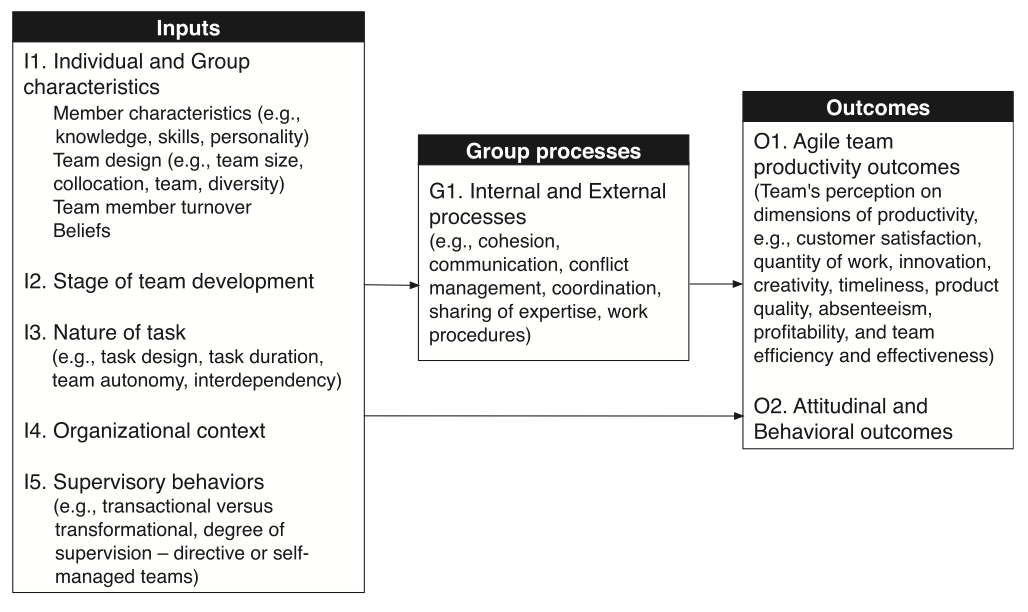
\includegraphics[width=150mm]{images/IPO.png}
\caption{Agile team productivity conceptual framework.}
\label{atpcf}
\end{figure}

After collecting the data from their multi-case study they mapped the results in a thematic map on agile productivity factors. These findings showed three main groups of team management and their impact on productivity. For this study it is the ``Inter-team coordination'' and ``Team design choices'' that are interesting because of their impact on coordination to a larger degree, meaning ``Team member turnover'' is left out. 

In ``Team design choices'' four roots of impact were identified: ``Team size'', ``Team members skills'', ``Team collocation'' and ``Team members allocation''. Out of these team collocation and team size seem to effect coordination effectiveness the most. Their findings showed that smaller teams led to better communication and alignment, while collocation had a positive influence on team productivity as it helped overcome invisible barriers between teams in a hierarchical company.

For ``Inter-team coordination'' two roots were identified: ``Lack of commitment among teams'' and ``Inappropriate coordination rules among teams''. One of the main reasons for negative impact was identified to be external dependencies because projects often were left waiting for results of entities outside the project team. So a problem in inter-team coordination was misalignment, hence, synchronisation is an important factor.

\subsubsection{Dispersion, Coordination and Performance in Global Software Teams: A Systematic Review}

Anh et al. performed a systematic literature review (SLR) to collect relevant studies on dispersion, coordination and performance in global software development (GSD), and highlighted the findings of impact factors in a thematic mapping \cite{Anh2012}. It is important to note that the findings are not from agile software development, but they are still interesting because of the global aspect in the literature used. The results are briefly summarised in table \ref{GSD}:

\begin{table}
\begin{center}
    \begin{tabular}{ | p{5cm} | p{8cm} |}
    \hline
    \textbf{Type} & \textbf{Impact on team performance} \\ \hline
    Presence of geographical dispersion & Negative (work takes longer time, less effective communication and coordination) \\ \hline
    Number of sites/Team size & Negative (complicates coordination and hampers communication) \\ \hline
    Large time zone differences between teams & Negative (creates coordination problems because of the complexity introduced) \\ \hline
    \end{tabular}
    \caption{Impact of geographical dispersion on performance.}
    \label{GSD}
\end{center}
\end{table}

\subsubsection{Team Performance in Agile Development Teams: Findings from 18 Focus Groups}

Dingsøyr and Lindsjørn carried out a focus group study looking at which factors the agile software practitioners in the research perceived as influential on effective teamwork \cite{Dingsoyr2013c}. This paper focuses on the team performance of individual teams, but is included because of its agile nature. To place the suggestions from the participants into categorise Dingsøyr et al. decided to use the ``Big Five'' model proposed by Salas et al. \cite{Salas2005} leading to eight teamwork components: ``Team leadership'', ``Mutual performance monitoring'', ``Backup behaviour'', ``Adaptability'', ``Team orientation'', ``Shared mental models'', ``Mutual trust'' and ``Closed-loop communication''. A summary of the distribution of all suggestions over these components is outlined in table \ref{summary2}.

\begin{table}
\begin{center}
    \begin{tabular}{ | p{6cm} | p{2.5cm} | p{2.5cm} | p{2.5cm} |}
    \hline
    \textbf{Teamwork component} & \textbf{Foster} & \textbf{Hinder} & \textbf{Total} \\ \hline
    Team leadership & 90 & 139 & 229 \\ \hline
    Mutual performance monitoring & 49 & 22 & 71 \\ \hline
    Backup behaviour & 44 & 57 & 101 \\ \hline
    Adaptability & 46 & 50 & 96 \\ \hline
    Team orientation & 91 & 65 & 156 \\ \hline
    Shared mental models & 104 & 59 & 163 \\ \hline
    Mutual trust & 97 & 58 & 155 \\ \hline
    Closed-loop communication & 122 & 90 & 212 \\ \hline
    Sum & 643 & 540 & 1183 \\ \hline
    \end{tabular}
    \caption{Summary of the distribution of suggestions over teamwork components.}
    \label{summary2}
\end{center}
\end{table}

The teamwork component with the strongest connection to coordination is ``closed-loop communication''. Looking at table \ref{summary2} a lot of emphasis was aimed towards the component from the practitioners (second highest total count). This again illustrates the importance of coordination. The sub-components identified of closed-loop communication are outlined in table \ref{closedloop}.

\begin{table}
\begin{center}
    \begin{tabular}{ | p{4cm} | p{5.25cm} | p{5.25cm} |}
    \hline
    \textbf{Sub-component} & \textbf{Foster} & \textbf{Hinder} \\ \hline
    Co-location & Physical presence \newline Co-location \newline Physically placed together & People are distributed \newline Distance \newline Not co-located \\ \hline
    Openness & Open communication \newline Openness in the team \newline Open dialogue & Secrecy \newline Retaining information \\ \hline
    Infrastructure & Process support tools \newline Suitable office spaces \newline Tools that work & Bad tools \newline Bad office facilities \\ \hline
    Visualising status and progress & Informative workspace \newline Visualise things that go well \newline Whiteboard/task-board & No whiteboards \\ \hline
    Social atmosphere & Good atmosphere \newline Fun \newline Friendly tone & Scolding \newline Antisocial environment \newline Bad atmosphere \\ \hline
    \end{tabular}
    \caption{Sub-components identified of closed-loop communication with their respective performance items.}
    \label{closedloop}
\end{center}
\end{table}

As can be seen from table \ref{closedloop} a lot of attention was directed towards location of team members, infrastructure and supportive tools, and organisational culture. The presence of co-location, a good infrastructure and supportive tools, and an open and social climate seem to all have a positive effect on team effectiveness.

\subsubsection{Summary}

The findings from the different studies are summarised in table \ref{summary}. Note that it could be argued that misalignment and synchronisation, as well as team collocation and presence of geographical dispersion, are contrasts of each other. They are however included in the summary table because they were identified as important aspects in the different studies.

\begin{table}
\begin{center}
    \begin{tabular}{ | p{8cm} | p{6cm} |}
    \hline
    \textbf{Type} & \textbf{Impact} \\ \hline
    Organisational openness culture & \textcolor{ForestGreen}{Positive} \\ \hline
    Misalignment & \textcolor{red}{Negative} \\ \hline
    Synchronisation & \textcolor{ForestGreen}{Positive} \\ \hline
    Team co-location & \textcolor{ForestGreen}{Positive} \\ \hline
    Presence of geographical dispersion & \textcolor{red}{Negative} \\ \hline
    Number of sites/Team size & \textcolor{red}{Negative} \\ \hline
    Large time zone differences between teams & \textcolor{red}{Negative} \\ \hline
    Infrastructure/Supportive tools & \textcolor{ForestGreen}{Positive} \\ \hline
    \end{tabular}
    \caption{Summary of impacts identified in the studies.}
    \label{summary}
\end{center}
\end{table}

\section{Shared Mental Models}

%TODO: Trust, Shared Mental Models (Cannon-Bowers et al. 1993, http://www-management.wharton.upenn.edu/klein/documents/Lim_Klein_Team_mental_models_2006.pdf,  task model, team model and team interaction model)

%TODO: Sitering: Cannon-Bowers 1990, Cannon-Bowers 1993, Rouse and Morris 1986, Mathieu 2000, Yu 2014

Shared (or team) mental models was originally proposed by Cannon-Bowers et al. in 1990 \cite{}, building on prior research in cognitive psychology on individuals’ mental models. Rouse et al. \cite{} defined the mental model of an individual as a ``mechanism whereby humans generate descriptions of system purpose and form, explanations of system functioning and observed system states, and predictions of future system states''. Hence, the mental model of a human-being can be seen as that individual's perception of the world, or put in other words, his reality. In similar fashion to individuals' mental model, Cannon-Bowers et al. propose that team members have shared mental models in regards to the equipment, interaction patterns, team procedures etc. within their respective teams. Below their definition of a shared mental model is outlined:

\begin{fancyquotes}
Knowledge structures held by members of a team that enable them to form accurate explanations and expectations for the task, and, in turn, to coordinate their actions and adapt their behaviour to demands of the task and other team members \cite{}.
\end{fancyquotes}

Cannon-Bowers et al. \cite{} goes on to suggest four shared mental models (or team mental models as they called them) that should be present to achieve a higher degree of team effectiveness: ``equipment model'', ``task model'', ``team interaction model'' and ``team model''. Firstly the ``equipment model'' is concerned with the technology used by the team to perform their team tasks, and their shared understanding of this technology. The ``task model'' looks at how team members perceive the team procedures, strategies, environmental conditions, and task contingencies. The third mental model described by Cannon-Bowers et al. is the ``team interaction model'' which captures how members understand their own and other team personnels' responsibilities, norms, and interaction patterns. The last model suggested is the ``team model'' which reflects how team members understand the others' skills, attitudes, knowledge, strengths and weaknesses.

Mathieu et al. \cite{} however argued that these four team mental models suggested by Cannon-Bowers et al. \cite{} could be divided and categorised into two areas. The first of these he called ``task-work'' containing the ``equipment'' and ``task'' models, and the second labelled ``teamwork'' including the ``team interaction'' and ``team'' models. The ``task-work'' mental models describe how team members' mental models are structured in regards to the equipment and procedures used to carry out their tasks. The ``teamwork'' mental models on the other hand outline how team members' mental models are structured in regards to team interaction processes and the perception of other team members' knowledge. In the study by Mathieu et al. \cite{} they found that both task-work mental model similarity and teamwork mental model similarity were notably positively related to team process, e.g., communication, cooperation and coordination, which in turn were to a large degree associated to team performance.

Yu et al. \cite{} also performed a conceptual analysis using shared mental model theory as a lens to examine three agile practices from Xtreme Programming (XP) and Scrum (system metaphor, stand-up meeting, and on-site customer). The objective of their research was to examine and understand how agile methodology practices enable software development teams to accomplish effective teamwork. In a short summary their work shows that the creation of shared mental models is one of the main benefits that agile development methodologies and practices brings with them, where the main benefit is enabling better collaboration within the teams. Their work demonstrates that the analysed agile practices assist the progress of the four stages of shared mental model development: knowing, learning, understanding and executing. Further, the research shows how agile practices contribute to achieving the two earlier mentioned shared mental models: teamwork and task-work.

\section{Mutual Trust}

%A teamwork model for understanding an agile team: A case study of a Scrum project
%http://www.uio.no/studier/emner/matnat/ifi/INF5181/h14/artikler-teamarbeid/salas_etal_2005_is_there_a_big_five_in_teamwork---copy.pdf
% http://onlinelibrary.wiley.com/doi/10.1111/j.1467-8608.2008.00517.x/full
%Webber, S. S. (2002). Leadership and trust facilitating cross-functional team success. Journal of Management Development, 21, 201-214.
%Bandow, D. (2001). Time to create sound teamwork. The Journal for Quality and Participation, 24, 41-47.
%Cooper, R., & Sawaf, A. (1996). Executive EQ: Emotional intelligence in leadership and organizations. New York: Grosset/Putnam.
% McEvily, B. and Marcus, A. 2005. ‘Embedded ties and the acquisition of competitive capabilities. Strategic Management Journal, 26:11, 1033–1055. 
%Trust, coordination and knowledge flows in R&D projects: the case of fuel cell technologies, Stian Nygaard and Angeloantonio Russo, 27 DEC 2007

Trust has been an aspect brought up by several researchers and seems to be closely linked to the previously described shared mental models. The general thoughts on mutual trust seems to be that it is an important aspect for achieving efficient teams and coordination within and across teams. However, a lot of these researchers use different definitions of the word. In this work the definition of trust used is the one Sheila Simsarian Webber provided in 2002:

\begin{fancyquotes}
The shared perception that individuals in the team will perform particular actions important to its members and will recognisee and protect the rights and interests of all the team members engaged in their joint endeavour.
\end{fancyquotes}

One of the more recognised papers on teamwork by Salas et al. highlights the importance of mutual trust. In their work they describe a set of ``Big Five'' which generates teamwork, however they stress that these five dimensions can not function without three supporting and coordinating mechanisms. These three coordinating mechanisms are namely shared mental models, mutual trust and engagement in closed-loop communication. A graphical representation of their model can be witnessed in figure \ref{salas}, but will not be further explained.

\begin{figure}
\centering
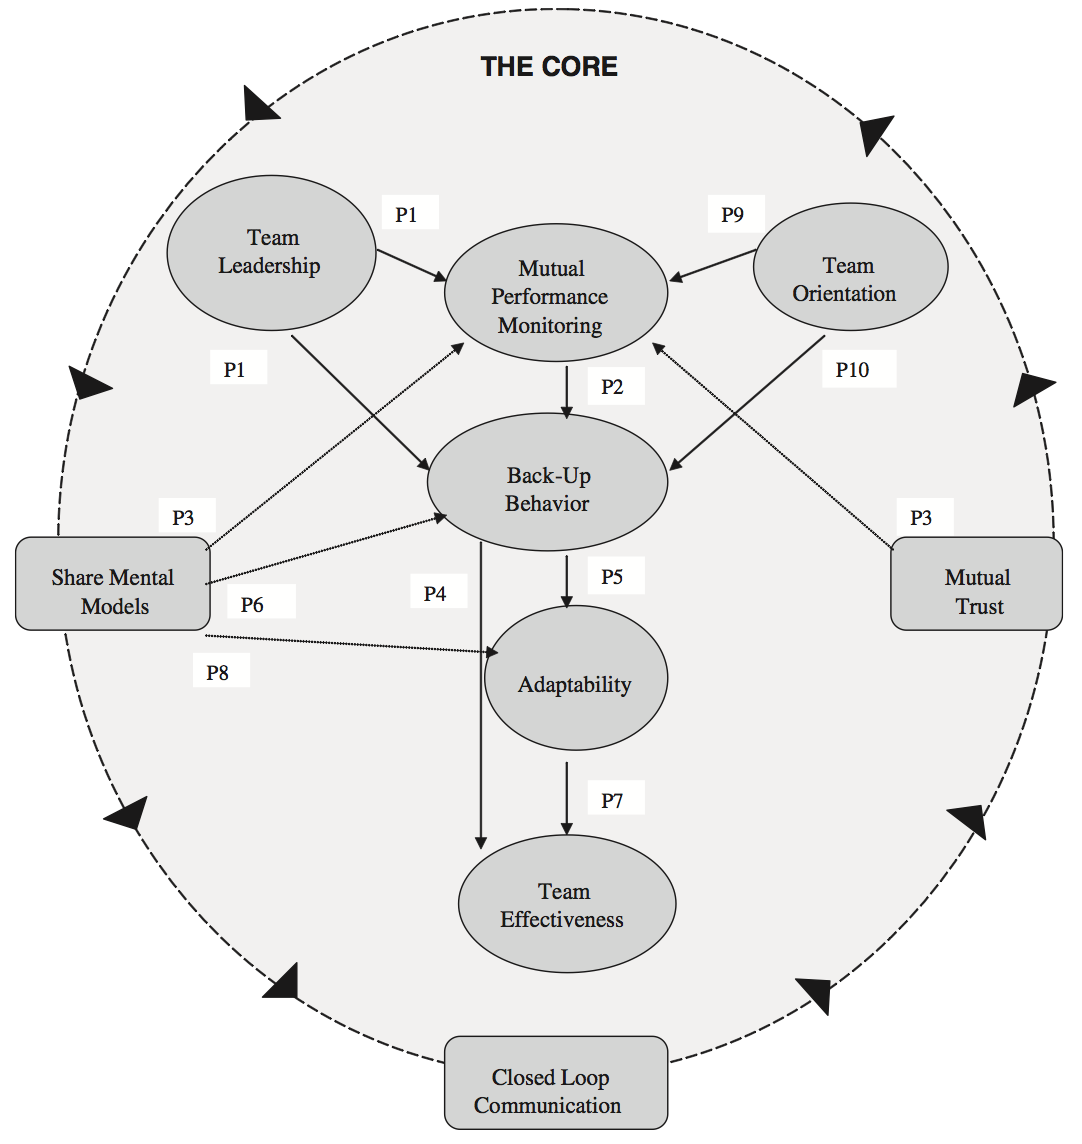
\includegraphics[width=150mm]{images/salas.png}
\caption{Graphical representation of the ``Big Five'' and supporting coordination mechanisms.}
\label{salas}
\end{figure}

There has been identified several impacts that trust can have on teams and team members. Bandow published a research on teamwork where she highlighted that trust affected several team processes and outcomes, e.g., membership contribution, team participation, product quality and cycle time. She further outlined that it is important that team members feel that their voice is heard, if not they will most likely be less willing to share their opinions and information. As a worst case scenario this might even lead to members not participating in information sharing arenas as they fear other members will perceive them as incompetent \cite{Bandow}. Also, without sufficient trust the team members might waste time and effort on checking each other as opposed to collaborating \cite{Cooper}. In general achieving mutual trust within projects seems to allow for information to flow more freely between the members. Without it there is a big chance it could spiral negatively and grow in concern where productivity goes down.

Similar findings to Salas et al. \cite{salas} were identified by Moe et al. \cite{moe} when they carried out a case study on a Scrum project. They state that ``without sufficient trust, team members will expend time and energy protecting, checking and inspecting each other as opposed to collaborating to provide value-added ideas. It is evident that trust is a prerequisite for shared leadership, feedback, and communication. Our finding regarding the lack of trust also confirms previous research on trust \cite{bandow}, such that team members may not be willing to share information if they fear being perceived as incompetent.". This highlights that trust is also identified as an important aspect in agile development.

Trust was also identified as a key factor both in small and large R\&D projects by Nygaard et al. \cite{}. They argue that small projects generally have a high level of trust because of the tight connections witnessed between partners and coordination benefits, while the larger projects usually benefit from having a high degree of variety in knowledge sources. They state that trust is a key factor for explaining exchange of knowledge and the creation of coordination benefits for organisations in most industries. They state that trust among partners supporting coordination and the aforementioned variety of knowledge flows within the projects is of uttermost importance to increase the likelihood of success. They back their work up by pointing to previous literature on similar research by McEvily et al. \cite{}.